% 第3章第4节：输运方程与传播（特征线与初值解；守恒形式与间断）。

\section{输运方程与传播}
\label{sec:pde-transport}

扩散把场抹平，输运则把场搬走。本节研究给定速度场怎样搬运一个初始场。关键的想法是跟着流动走：沿着速度场的轨迹，偏微分方程变成上一章的常微分方程。我们还要区分两种搬运：搬运的是场的数值（如染料的颜色），还是场所代表的质量（如染料的浓度）；最后看到，当速度依赖场本身时，轨迹会相撞，光滑的解会在有限时间内破裂。

\subsection{特征线与初值解}
\label{sec:pde-characteristics}

\paragraph{常速度平移}
想象一条以恒定速度$b$流动的河，水中溶有一种示踪物，$u(x,t)$是它在位置$x$、时刻$t$的颜色深浅。示踪物不扩散，只随水流走，于是\term{输运方程}（transport equation）
\begin{equation}
  u_t+bu_x=0,\qquad u(x,0)=u_0(x)
  \label{eq:pde-transport-constant}
\end{equation}
描述它的变化。站在岸上看，某处的颜色在变；坐在随水漂流的小船上看，周围的颜色不变。设小船位置为$X(t)=y+bt$，由链式法则
\[
  \frac{\mathrm d}{\mathrm dt}u(X(t),t)=u_x(X(t),t)\,X'(t)+u_t(X(t),t)=bu_x+u_t=0,
\]
所以$u$沿着这条线保持初值$u_0(y)$。给定$(x,t)$，反解出出发点$y=x-bt$，得$u(x,t)=u_0(x-bt)$。若$u_0\in C^1(\mathbb R)$，直接求导可验证它是经典解；上面的推导同时说明任何$C^1$解都必须是它，所以解唯一。

在$(x,t)$平面中，直线$x-bt=y$称为\term{特征线}（characteristic）。图~\ref{fig:pde-characteristics}(a)画出了这些平行直线，颜色是解的值：鼓包沿特征线原封不动地平移。

\begin{figure}[!htb]
  \centering
  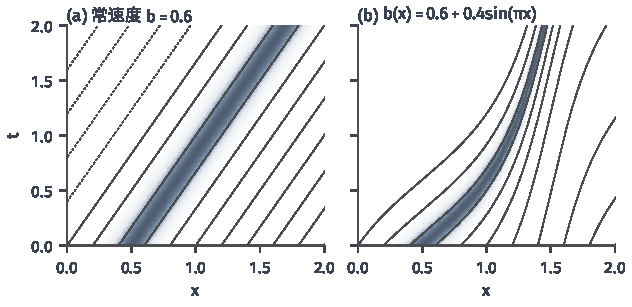
\includegraphics[width=107mm]{figures/03-optimization-evolution-and-signals/02-processes-and-trajectory-evolution/matplotlib/pde-characteristics/figure.pdf}
  \caption{输运方程$u_t+b(x)u_x=0$在$[0,2]$上的特征线（细线）与解（颜色越深值越大），初值$u_0=\exp(-((x-0.5)/0.15)^2)$，左端流入边界上给定$u(0,t)=0$。(a)~常速度$b=0.6$：特征线是平行直线，实线从$t=0$出发，虚线从流入边界出发。(b)~$b(x)=0.6+0.4\sin(\pi x)$：特征线在速度快处变陡，在$x=1.5$附近速度最慢处聚拢，鼓包沿途保持高度、宽度被压缩。特征线由四阶Runge--Kutta法积分。}
  \label{fig:pde-characteristics}
\end{figure}

\paragraph{变速度场与特征线方程}
速度随位置和时间变化时，小船的轨迹不再是直线，但道理相同。在$\mathbb R^d$中考虑
\begin{equation}
  u_t+\bm b(\bm x,t)\cdot\nabla u=0,\qquad u(\bm x,0)=u_0(\bm x).
  \label{eq:pde-transport}
\end{equation}
沿着曲线$\bm X(t)$，$\frac{\mathrm d}{\mathrm dt}u(\bm X(t),t)=\nabla u\cdot\bm X'+u_t$，它为零的条件正是$\bm X'=\bm b(\bm X,t)$。所以特征线就是速度场的轨线：
\begin{equation}
  \dot{\bm X}(t)=\bm b(\bm X(t),t),\qquad\bm X(0)=\bm y .
  \label{eq:pde-characteristic-ode}
\end{equation}
这是第~\ref{chap:ordinary-differential-equations}章的初值问题。若$\bm b$连续、关于$\bm x$连续可微且$D_{\bm x}\bm b$有界，则它关于$\bm x$整体Lipschitz，对每个$\bm y$有定义在全部$t\geq0$上的唯一解。记$\Phi_t(\bm y)=\bm X(t)$为时刻$t$的流映射。由唯一性，从时刻$t$的点$\bm x$反向求解式~\eqref{eq:pde-characteristic-ode}得到唯一的出发点，所以$\Phi_t$是$\mathbb R^d$上的双射；并且$\bm b$关于$\bm x$连续可微时，流映射及其逆关于初值连续可微，这是可微依赖定理的结论，这里引用而不证明。

\begin{theorem}[输运方程的特征线解]
\label{thm:pde-transport-characteristics}
设$\bm b$满足上述条件，$u_0\in C^1(\mathbb R^d)$。则$u(\bm x,t)=u_0\bigl(\Phi_t^{-1}(\bm x)\bigr)$是式~\eqref{eq:pde-transport}的唯一$C^1$解。
\end{theorem}

\begin{proof}
唯一性：若$u$是$C^1$解，上面的链式法则说明$u(\Phi_t(\bm y),t)$关于$t$的导数为零，所以$u(\Phi_t(\bm y),t)=u_0(\bm y)$；每个$(\bm x,t)$都在唯一一条特征线上，取$\bm y=\Phi_t^{-1}(\bm x)$即得公式。存在性：公式定义的$u$是$C^1$函数的复合，连续可微；沿每条特征线它等于常数$u_0(\bm y)$，对$t$求导即得在点$(\Phi_t(\bm y),t)$处$u_t+\bm b\cdot\nabla u=0$，而这些点覆盖了整个$\mathbb R^d\times[0,\infty)$。
\end{proof}

解的值沿特征线不变，但形状可以变。一维时取$b(x)=x$，特征线$X=ye^t$，解$u=u_0(xe^{-t})$：初值被横向拉伸$e^t$倍，高度不变。图~\ref{fig:pde-characteristics}(b)中速度先快后慢，鼓包进入慢速区时前端先减速、后端追上来，于是被压窄。

\paragraph{源项沿特征线累计}
若示踪物在流动中还被注入或分解，方程变为$u_t+\bm b\cdot\nabla u=s(\bm x,t)$。沿特征线，$\frac{\mathrm d}{\mathrm dt}u(\bm X(t),t)=s(\bm X(t),t)$，积分得
\[
  u\bigl(\Phi_t(\bm y),t\bigr)=u_0(\bm y)+\int_0^ts\bigl(\Phi_\tau(\bm y),\tau\bigr)\,\mathrm d\tau .
\]
例如$b=1$、$s=1$时$u=u_0(x-t)+t$：小船上的人看到颜色每单位时间加深$1$。若还有按比例的分解$-cu$，沿特征线就得到线性常微分方程$U'=-cU+s$，用常数变易法求解。输运方程于是化为一族以出发点$\bm y$为参数的常微分方程，每条特征线各自独立地计算。

\paragraph{有界区域：只在流入边界给数据}
在区间$(0,1)$上取$b=1$。特征线从左端流入，从右端流出。初值$u_0$只决定从底边出发的特征线上的值；从左端$x=0$进入的特征线还需要另外的数据，所以给定$u(0,t)=g(t)$，解为
\[
  u(x,t)=\begin{cases}u_0(x-t),&x\geq t,\\ g(t-x),&x<t .\end{cases}
\]
右端$x=1$处的值已经被沿特征线搬来的数据决定，再规定它会与之冲突。一般地，边界上只能在\term{流入边界}（inflow boundary）$\{\bm x\in\partial\Omega:\bm b\cdot\bm n<0\}$给数据，这与热方程在整个边界上给数据完全不同。若$u_0(0)\neq g(0)$，解在特征线$x=t$上有一个跳跃，它被原样搬向下游，永不磨光，这与第~\ref{sec:pde-boundary-solution-meaning}小节关于相容条件的讨论相呼应。图~\ref{fig:pde-characteristics}中的虚线就是从流入边界出发的特征线，那里的值来自$g=0$。

\paragraph{反向追踪的条件}
公式$u_0(\Phi_t^{-1}(\bm x))$依赖于每个点恰好有一条特征线经过。速度场不够正则时，这一点可以失败。取$b(x)=2\sqrt{|x|}$，它连续但在原点不满足Lipschitz条件。从原点出发，$X\equiv0$与$X=t^2$都是$X'=2\sqrt{|X|}$的解；还可以在原点停留任意时间$\tau$后再出发，$X=(t-\tau)^2$。从$x>0$、$t>\sqrt x$的点反向追踪，可以回到$y=0$，也可以经过原点后回到任何$y\in[-(t-\sqrt x)^2,0]$。于是$u(x,t)$等于$u_0$在这些点中哪一处的值无法确定，输运方程有多个解。特征线方法的使用条件就是流映射存在、唯一，并且特征线覆盖了需要求解的区域。

\subsection{守恒形式与间断}
\label{sec:pde-conservation}

\paragraph{搬运数值与搬运质量}
前面的$u$是一种“标签”：颜色深浅随水移动，但不关心水被压缩还是拉伸。若要描述的是单位体积中的质量，即密度$\rho$，压缩的水流会让密度升高。用第~\ref{sec:pde-heat-modes}小节同样的守恒推理，区域内质量的变化等于穿过边界的通量$\rho\bm b$，得到\term{连续性方程}（continuity equation）
\begin{equation}
  \rho_t+\nabla\cdot(\bm b\rho)=0 .
  \label{eq:pde-continuity}
\end{equation}
展开散度，$\nabla\cdot(\bm b\rho)=\bm b\cdot\nabla\rho+\rho\nabla\cdot\bm b$，所以沿特征线
\[
  \frac{\mathrm d}{\mathrm dt}\rho\bigl(\bm X(t),t\bigr)=-\rho\,\nabla\cdot\bm b .
\]
与式~\eqref{eq:pde-transport}对比，差别只在散度一项：流动压缩（$\nabla\cdot\bm b<0$）处密度沿途增加，流动扩张处密度减少；速度场无散度时两个方程相同。式~\eqref{eq:pde-continuity}的通量写在散度号里，称为\term{守恒形式}（conservative form）。

数值不变与质量不变是两个不同的守恒性质。设$A$为一块初始区域，$\Phi_t(A)$是它随流运动到时刻$t$的位置，下面证明$\int_{\Phi_t(A)}\rho\,\mathrm d\bm x$不随时间变化。令$J_t(\bm y)=\det D\Phi_t(\bm y)$。$D\Phi_t$满足变分方程$\frac{\mathrm d}{\mathrm dt}D\Phi_t=D_{\bm x}\bm b(\Phi_t,t)\,D\Phi_t$，由行列式求导公式$\frac{\mathrm d}{\mathrm dt}\det\bm M=\det\bm M\operatorname{tr}(\bm M^{-1}\bm M')$，得$\frac{\mathrm d}{\mathrm dt}J_t=(\nabla\cdot\bm b)(\Phi_t,t)\,J_t$，且$J_0=1$，所以$J_t>0$。换元得
\[
  \int_{\Phi_t(A)}\rho(\bm x,t)\,\mathrm d\bm x=\int_A\rho\bigl(\Phi_t(\bm y),t\bigr)J_t(\bm y)\,\mathrm d\bm y,
\]
被积函数对$t$的导数是$J_t\bigl(\frac{\mathrm d}{\mathrm dt}\rho+\rho\nabla\cdot\bm b\bigr)=0$。体积被压缩多少，密度就升高多少，二者乘积不变。

\begin{example}[收缩流中的数值与密度]
\label{ex:pde-compressing-flow}
取一维速度$b(x)=-x$，流体向原点收缩，特征线$X=ye^{-t}$。数值方程$u_t-xu_x=0$的解为$u=u_0(xe^t)$：形状横向压缩$e^t$倍，高度不变。连续性方程$\rho_t-(x\rho)_x=0$中$\nabla\cdot b=-1$，沿特征线$\frac{\mathrm d}{\mathrm dt}\rho=\rho$，所以$\rho(x,t)=e^t\rho_0(xe^t)$：形状同样被压缩，高度却升高$e^t$倍，总质量$\int\rho\,\mathrm dx=\int\rho_0\,\mathrm dx$不变。
\end{example}

图~\ref{fig:pde-transport-vs-continuity}把这两种搬运并排画出。若把一个随机初始状态放进常微分方程演化，它的概率密度满足的正是连续性方程；第~\ref{chap:continuous-time-stochastic-processes}章在加入随机扰动后会得到相应的密度方程。

\begin{figure}[!htb]
  \centering
  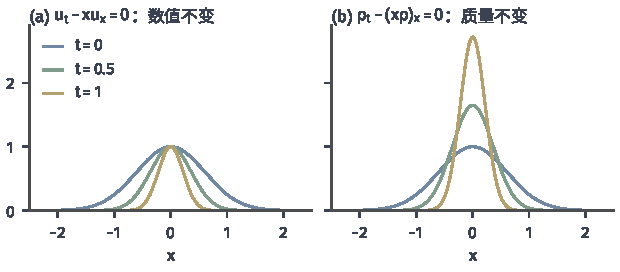
\includegraphics[width=105mm]{figures/03-optimization-evolution-and-signals/02-processes-and-trajectory-evolution/matplotlib/pde-transport-vs-continuity/figure.pdf}
  \caption{收缩速度场$b(x)=-x$下的两种搬运（例~\ref{ex:pde-compressing-flow}），初值同为$\exp(-x^2/0.72)$，三种颜色依次为$t=0,0.5,1$。(a)~输运方程：数值沿特征线不变，峰高保持$1$。(b)~连续性方程：峰高依次为$1$、$e^{0.5}\approx1.65$、$e\approx2.72$，曲线下面积保持约$1.504$。}
  \label{fig:pde-transport-vs-continuity}
\end{figure}

\paragraph{积分形式的守恒律}
在一维中，许多守恒量满足形如
\begin{equation}
  u_t+\bigl(F(u)\bigr)_x=0
  \label{eq:pde-conservation-law}
\end{equation}
的方程，称为\term{守恒律}（conservation law），$F$是通量函数。线性输运对应$F(u)=bu$；交通流中$u$是车辆密度，$F(u)=u\,v(u)$，车速$v$随密度增大而降低。式~\eqref{eq:pde-conservation-law}来自积分形式
\[
  \frac{\mathrm d}{\mathrm dt}\int_a^bu\,\mathrm dx=F\bigl(u(a,t)\bigr)-F\bigl(u(b,t)\bigr),
\]
即区间内的总量变化等于左端流入减右端流出。积分形式只要求$u$可积，对有跳跃的$u$也有意义；微分形式需要$u$可微。下面会看到，这个区别在非线性情形中不可回避。

\paragraph{Burgers方程中的特征线交叉}
取$F(u)=u^2/2$，对光滑的$u$，式~\eqref{eq:pde-conservation-law}即\allowbreak\term{Burgers方程}（Burgers' equation）$u_t+uu_x=0$。它与输运方程的区别是：速度不再是给定的$b$，而是$u$本身。沿用小船的论证，特征线满足$X'=u(X,t)$，而$u$沿特征线不变，所以特征线仍是直线
\[
  X(t)=y+u_0(y)\,t,
\]
只是不同出发点的直线斜率不同：值大的点跑得快。若$u_0$在某处递减，后面跑得快的点就会追上前面跑得慢的点。

固定$t$，映射$y\mapsto y+u_0(y)t$的导数是$1+u_0'(y)t$。只要它保持为正，特征线不相交，$u$由$u_0$经此映射的逆唯一确定，并且由$u(X(t),t)=u_0(y)$对$y$求导得$u_x=u_0'(y)/(1+u_0'(y)t)$。若$u_0'$在某处为负，最早在
\[
  t_*=\frac1{\max_y\bigl(-u_0'(y)\bigr)}
\]
时刻，导数$1+u_0'(y)t$在使$-u_0'$最大的点处变为零，$u_x$趋于$-\infty$：初值再光滑，经典解也在有限时间内失效。取$u_0=e^{-x^2}$，$-u_0'=2xe^{-x^2}$在$y=1/\sqrt2$处取最大值$\sqrt2e^{-1/2}\approx0.858$，所以$t_*\approx1.166$，交叉发生在$x=y+u_0(y)t_*=\sqrt2$。图~\ref{fig:pde-burgers}(a)画出了这些特征线：鼓包后坡的直线在$t_*$处开始交叉。

过了$t_*$，若仍沿特征线搬运数值，同一个$x$会被几条特征线带来不同的值，剖面变成图~\ref{fig:pde-burgers}(b)中虚线那样的S形，不再是函数的图像。物理上，前方的车辆堆积时不会穿过彼此，而是形成一个密度跳跃。我们需要允许间断的解。

\begin{figure}[!htb]
  \centering
  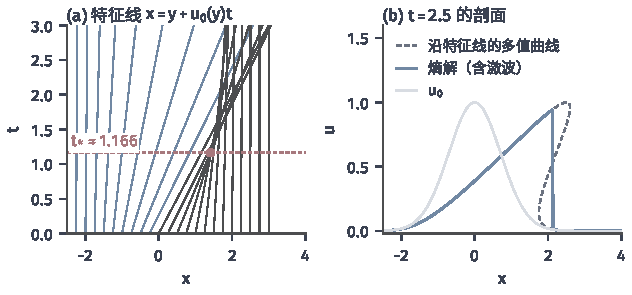
\includegraphics[width=107mm]{figures/03-optimization-evolution-and-signals/02-processes-and-trajectory-evolution/matplotlib/pde-burgers/figure.pdf}
  \caption{Burgers方程$u_t+(u^2/2)_x=0$，初值$u_0=e^{-x^2}$。(a)~特征线$x=y+u_0(y)t$，蓝色从$y<0$出发、深灰色从$y\geq0$出发；圆点为最早的交叉点$(\sqrt2,t_*)$，$t_*\approx1.166$。(b)~$t=2.5$时的剖面：虚线是沿特征线搬运得到的多值曲线；实线是用Godunov有限体积格式（$4000$个网格，CFL数$0.45$）计算的熵解，在$x\approx2.12$处有激波；浅灰线是初值。}
  \label{fig:pde-burgers}
\end{figure}

\paragraph{弱解、Rankine--Hugoniot条件与熵条件}
对光滑解，用$\varphi\in C_c^1(\mathbb R\times[0,\infty))$乘以式~\eqref{eq:pde-conservation-law}并在$x$与$t$上分部积分，得到
\[
  \int_0^\infty\!\!\int_{\mathbb R}\bigl(u\varphi_t+F(u)\varphi_x\bigr)\,\mathrm dx\,\mathrm dt+\int_{\mathbb R}u_0(x)\varphi(x,0)\,\mathrm dx=0 .
\]
导数全部转移到了测试函数上，这个式子对有界可测的$u$也有意义。称对所有这样的$\varphi$满足上式的$u$为守恒律的弱解，这与第~\ref{sec:pde-weak-form}小节的想法相同。

弱解允许跳跃，但跳跃不能随意移动。设解在$x=s(t)$处有一个跳跃，左侧值$u_L$、右侧值$u_R$。在包含$s(t)$的小区间$[a,b]$上用积分形式，区间很短时两侧近似为常数，总量约为$(s-a)u_L+(b-s)u_R$，它对$t$的导数为$s'(u_L-u_R)$，必须等于$F(u_L)-F(u_R)$。于是得到\term{Rankine--Hugoniot条件}（Rankine--Hugoniot condition）
\[
  s'(t)=\frac{F(u_L)-F(u_R)}{u_L-u_R} .
\]
对Burgers方程，$s'=(u_L+u_R)/2$，跳跃以两侧值的平均速度移动。这样移动的跳跃称为\term{激波}（shock wave）。

可是弱解不一定唯一。取初值在$x<0$为$0$、在$x>0$为$1$。一方面，$u_L=0$、$u_R=1$的跳跃以速度$1/2$移动，满足Rankine--Hugoniot条件，是一个弱解。另一方面，令$u=0$（$x<0$），$u=x/t$（$0\leq x\leq t$），$u=1$（$x>t$），直接验证$u_t+uu_x=-x/t^2+(x/t)(1/t)=0$，它连续且是另一个弱解，称为\term{稀疏波}（rarefaction wave）。需要额外的选择规则。对凸的$F$，Lax提出的\term{熵条件}（entropy condition）要求两侧的特征线都流入激波：$F'(u_L)>s'>F'(u_R)$，对Burgers方程即$u_L>s'>u_R$。上例中$u_L=0<u_R=1$，跳跃违反熵条件，物理的解是稀疏波；反过来$u_L=1$、$u_R=0$的跳跃满足熵条件，是真正的激波。

满足熵条件的弱解也可以理解为加一点扩散再取极限：$u_t+uu_x=\varepsilon u_{xx}$在$\varepsilon\to0$时的解趋于熵解，激波是被极小的扩散磨成的一段陡峭过渡。图~\ref{fig:pde-burgers}(b)中的数值格式自带少量数值扩散，算出的正是熵解。非线性守恒律的熵解理论，包括一般通量下的存在唯一性，本章不展开；这里只需看到两点：非线性可以让光滑解在有限时间内产生间断，这时必须扩大解的范围，并补充选择物理解的条件。
